%% BioMed_Central_Tex_Template_v1.06
%%                                      %
%  bmc_article.tex            ver: 1.06 %
%                                       %

%%IMPORTANT: do not delete the first line of this template
%%It must be present to enable the BMC Submission system to
%%recognise this template!!

%%%%%%%%%%%%%%%%%%%%%%%%%%%%%%%%%%%%%%%%%
%%                                     %%
%%  LaTeX template for BioMed Central  %%
%%     journal article submissions     %%
%%                                     %%
%%          <8 June 2012>              %%
%%                                     %%
%%                                     %%
%%%%%%%%%%%%%%%%%%%%%%%%%%%%%%%%%%%%%%%%%


%%%%%%%%%%%%%%%%%%%%%%%%%%%%%%%%%%%%%%%%%%%%%%%%%%%%%%%%%%%%%%%%%%%%%
%%                                                                 %%
%% For instructions on how to fill out this Tex template           %%
%% document please refer to Readme.html and the instructions for   %%
%% authors page on the biomed central website                      %%
%% http://www.biomedcentral.com/info/authors/                      %%
%%                                                                 %%
%% Please do not use \input{...} to include other tex files.       %%
%% Submit your LaTeX manuscript as one .tex document.              %%
%%                                                                 %%
%% All additional figures and files should be attached             %%
%% separately and not embedded in the \TeX\ document itself.       %%
%%                                                                 %%
%% BioMed Central currently use the MikTex distribution of         %%
%% TeX for Windows) of TeX and LaTeX.  This is available from      %%
%% http://www.miktex.org                                           %%
%%                                                                 %%
%%%%%%%%%%%%%%%%%%%%%%%%%%%%%%%%%%%%%%%%%%%%%%%%%%%%%%%%%%%%%%%%%%%%%

%%% additional documentclass options:
%  [doublespacing]
%  [linenumbers]   - put the line numbers on margins

%%% loading packages, author definitions

\documentclass[twocolumn]{bmcart}% uncomment this for twocolumn layout and comment line below
%\documentclass{bmcart}

%%% Load packages
\usepackage{amsthm,amsmath}
\usepackage{siunitx}
\usepackage{mfirstuc}
%\RequirePackage{natbib}
\usepackage[colorinlistoftodos]{todonotes}
\RequirePackage{hyperref}
\usepackage[utf8]{inputenc} %unicode support
%\usepackage[applemac]{inputenc} %applemac support if unicode package fails
%\usepackage[latin1]{inputenc} %UNIX support if unicode package fails
\usepackage[htt]{hyphenat}

\usepackage{array}
\newcolumntype{L}[1]{>{\raggedright\let\newline\\\arraybackslash\hspace{0pt}}p{#1}}

%%%%%%%%%%%%%%%%%%%%%%%%%%%%%%%%%%%%%%%%%%%%%%%%%
%%                                             %%
%%  If you wish to display your graphics for   %%
%%  your own use using includegraphic or       %%
%%  includegraphics, then comment out the      %%
%%  following two lines of code.               %%
%%  NB: These line *must* be included when     %%
%%  submitting to BMC.                         %%
%%  All figure files must be submitted as      %%
%%  separate graphics through the BMC          %%
%%  submission process, not included in the    %%
%%  submitted article.                         %%
%%                                             %%
%%%%%%%%%%%%%%%%%%%%%%%%%%%%%%%%%%%%%%%%%%%%%%%%%


%\def\includegraphic{}
%\def\includegraphics{}

%%% Put your definitions there:
\startlocaldefs
\endlocaldefs


%%% Begin ...
\begin{document}

%%% Start of article front matter
\begin{frontmatter}

\begin{fmbox}
\dochead{Report from 2015 OHBM Hackathon (HI)}

%%%%%%%%%%%%%%%%%%%%%%%%%%%%%%%%%%%%%%%%%%%%%%
%%                                          %%
%% Enter the title of your article here     %%
%%                                          %%
%%%%%%%%%%%%%%%%%%%%%%%%%%%%%%%%%%%%%%%%%%%%%%

\title{Highly Comparable Time-Series Analysis in Nitime}
\vskip2ex
\projectURL{Project URL: \url{https://github.com/benfulcher/hctsa\_python}}

\author[
addressref={aff1},
corref={aff1},
email={ben.fulcher@monash.edu}
]{\inits{BDF} \fnm{Ben D.} \snm{Fulcher}}

%%%%%%%%%%%%%%%%%%%%%%%%%%%%%%%%%%%%%%%%%%%%%%
%%                                          %%
%% Enter the authors' addresses here        %%
%%                                          %%
%% Repeat \address commands as much as      %%
%% required.                                %%
%%                                          %%
%%%%%%%%%%%%%%%%%%%%%%%%%%%%%%%%%%%%%%%%%%%%%%

\address[id=aff1]{%
  \orgname{Monash Institute of Cognitive and Clinical Neurosciences, Monash
University},
  \city{Melbourne},
  \street{770 Blackburn Rd},
  \postcode{3168},
  %
  \cny{Australia}
}

%%%%%%%%%%%%%%%%%%%%%%%%%%%%%%%%%%%%%%%%%%%%%%
%%                                          %%
%% Enter short notes here                   %%
%%                                          %%
%% Short notes will be after addresses      %%
%% on first page.                           %%
%%                                          %%
%%%%%%%%%%%%%%%%%%%%%%%%%%%%%%%%%%%%%%%%%%%%%%

\begin{artnotes}
\end{artnotes}

%\end{fmbox}% comment this for two column layout

%%%%%%%%%%%%%%%%%%%%%%%%%%%%%%%%%%%%%%%%%%%%%%
%%                                          %%
%% The Abstract begins here                 %%
%%                                          %%
%% Please refer to the Instructions for     %%
%% authors on http://www.biomedcentral.com  %%
%% and include the section headings         %%
%% accordingly for your article type.       %%
%%                                          %%
%%%%%%%%%%%%%%%%%%%%%%%%%%%%%%%%%%%%%%%%%%%%%%

%\begin{abstractbox}

%\begin{abstract} % abstract
	
%Blank Abstract

%\end{abstract}



%%%%%%%%%%%%%%%%%%%%%%%%%%%%%%%%%%%%%%%%%%%%%%
%%                                          %%
%% The keywords begin here                  %%
%%                                          %%
%% Put each keyword in separate \kwd{}.     %%
%%                                          %%
%%%%%%%%%%%%%%%%%%%%%%%%%%%%%%%%%%%%%%%%%%%%%%

%\vskip1ex

%\projectURL{\url{https://github.com/benfulcher/hctsa\_python}}
%\projectURL{https://github.com/benfulcher/hctsa\_python}

% MSC classifications codes, if any
%\begin{keyword}[class=AMS]
%\kwd[Primary ]{}
%\kwd{}
%\kwd[; secondary ]{}
%\end{keyword}

%\end{abstractbox}
%
\end{fmbox}% uncomment this for twcolumn layout

\end{frontmatter}

%{\sffamily\bfseries\fontsize{10}{12}\selectfont Project URL: \url{https://github.com/benfulcher/hctsa\_python}}

%%% Import the body from pandoc formatted text
\section{Introduction}\label{introduction}

The aim of this project was to demonstrate that an existing Matlab-based
package for implementing thousands of time-series analysis methods,
\href{https://github.com/benfulcher/hctsa}{hctsa}
(\url{https://github.com/benfulcher/hctsa}), could be extended to a
python-based implementation, for potential future inclusion into
\href{http://nipy.org/nitime/}{Nitime} (\url{http://nipy.org/nitime/}).

Recent work has contributed a comprehensive library of over 35,000
pieces of diverse time-series data, and over 7,000 unique structural
features extracted from hundreds of different time-series analysis
methods \cite{Fulcher2013}, which can be explored through an associated
\href{www.comp-engine.org/timeseries}{website}
(\url{www.comp-engine.org/timeseries}) and implemented using the
Matlab-based code package,
\href{https://github.com/benfulcher/hctsa}{hctsa}. The \emph{hctsa}
software provides a systematic, algorithmic platform for computing a
wide range of structural properties from a single time series, including
basic statistics of the distribution, linear correlation structure,
stationarity, information theoretic and entropy measures, methods from
the physical nonlinear time-series analysis literature, linear and
nonlinear model fits, and others. Thus, hctsa can be used to map a time
series to a comprehensive vector of structural features and these
features can then be systematically compared to determine and interpret
the most useful features for a given scientific objective.

In order to apply highly comparative time-series analysis in the
neuroscience community, it would be desirable to implement some
time-series analysis methods into
\href{http://nipy.org/nitime/}{Nitime}, a python-based software package
for performing time-series analysis on neuroscience data. While the
Nitime data format supports unevenly sampled data, \emph{hctsa} does
not; although for evenly sampled data it is trivial to extract the data
vector from the Nitime Timeseries class and run important time-series
algorithms on these data vectors. Implementation of useful time-series
features into python, and potential integration with Nitime, would not
only facilitate their use by the neuroscience community, but also their
maintenance and development within an open source framework.

\section{Approach}\label{approach}

An illustration of the approach is shown in Fig. \ref{centfig}. Each
time series is converted to a vector of thousands of informative
features using the \emph{hctsa} package; machine learning methods can
then be used to determine the most useful features (e.g., that best
discriminate patient groups, and where in the brain the best
discrimination occurs). In this project, we wanted to demonstrate a
feasible pathway for incorporating these useful features into the Nitime
package.

\begin{figure}[h!]
  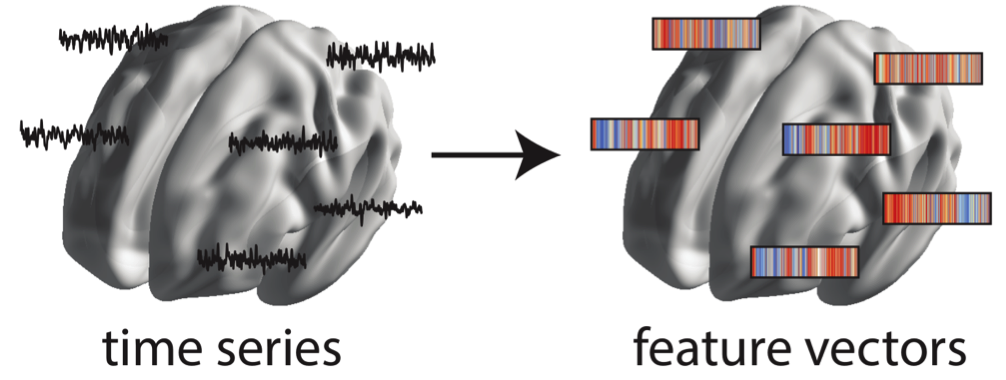
\includegraphics[width=.47\textwidth]{nitime.png}
  \caption{\label{centfig} Illustration of the highly comparative approach to time-series data from neuroscience.}
\end{figure}

\section{Results}\label{results}

I successfully implemented a handful of basic time-series analysis
functions from Matlab into python using partials, with basic support for
the Nitime data format. This proof-of-principle is
\href{https://github.com/benfulcher/hctsa_python}{here}.

\section{Conclusions}\label{conclusions}

Our results demonstrate that time-series analysis methods, discovered
using the \href{https://github.com/benfulcher/hctsa}{hctsa package}, can
be implemented natively in python in a systematic way, with support for
the time-series format used in Nitime. This will help facilitate future
work on time-series analysis to be incorporated straightforwardly into
an open source environment.

%%%%%%%%%%%%%%%%%%%%%%%%%%%%%%%%%%%%%%%%%%%%%%
%%                                          %%
%% Backmatter begins here                   %%
%%                                          %%
%%%%%%%%%%%%%%%%%%%%%%%%%%%%%%%%%%%%%%%%%%%%%%

\begin{backmatter}

\section*{Availability of Supporting Data}
More information about this project can be found at: \url{https://github.com/benfulcher/hctsa\_python}. Further data and files supporting this project are hosted in the \emph{GigaScience} repository REFXXX.

\section*{Competing interests}
None

\section*{Author's contributions}
BF wrote the software and the report.

\section*{Acknowledgements}
The authors would like to thank the organizers and attendees of the 2015
OHBM Hackathon.

  
  
%%%%%%%%%%%%%%%%%%%%%%%%%%%%%%%%%%%%%%%%%%%%%%%%%%%%%%%%%%%%%
%%                  The Bibliography                       %%
%%                                                         %%
%%  Bmc_mathpys.bst  will be used to                       %%
%%  create a .BBL file for submission.                     %%
%%  After submission of the .TEX file,                     %%
%%  you will be prompted to submit your .BBL file.         %%
%%                                                         %%
%%                                                         %%
%%  Note that the displayed Bibliography will not          %%
%%  necessarily be rendered by Latex exactly as specified  %%
%%  in the online Instructions for Authors.                %%
%%                                                         %%
%%%%%%%%%%%%%%%%%%%%%%%%%%%%%%%%%%%%%%%%%%%%%%%%%%%%%%%%%%%%%

% if your bibliography is in bibtex format, use those commands:
\bibliographystyle{bmc-mathphys} % Style BST file
\bibliography{brainhack-report} % Bibliography file (usually '*.bib' )

\end{backmatter}
\end{document}
